\chapter{Air Traffic Management}
\label{app:atm}

Earlier, in \cref{ch:atrds}, we did not focus as much on the particulars of the air traffic management problem specifically, as we were limited to a single airport case. However, when moving to the full network scenario, which has a lot more moving parts, we will need to take a closer look in order to develop a better understanding of how the different parts of the system come together, which will be of use when discussing further simulation building and modeling goals. Furthermore, we will also attempt to cover disruptions to air traffic networks in greater detail, to provide some preliminary background for modeling more complex effects. 

\section{National Airspace System}
\label{sec:atm-nas}

Let us briefly review the components and workings of the National Airspace System (NAS) at a high level view, before we go further in depth into the specific aspects of it that we are focused on. Specifically, we will base our study on information from the following FAA sources and defer to them for a more detailed and specific development: \cite{faa_nas_2023} for a more detailed coverage of flight rules and airspace classifications, as well as \cite{faa_tmi_2024} and \cite{faa_tfm_prez_2009} for more information on air traffic management. The NAS broadly refers to the network built from airspace relevant to domestic air travel, and includes various systems such as airports and landing areas, air navigation facilities, and procedures and regulations. These systems are responsible for maintaining safe and efficient operation of thousands of aircraft concurrently traveling through both controlled and uncontrolled airspace, with many different origins and destinations. We will be mainly focused on air traffic control (ATC) and air traffic management (ATM), which are closely interrelated.

\subsection{NAS Traffic Control}

The airspace over the United States is divided into sectors, also known as Flight Information Regions (FIRs), each managed by an Air Route Traffic Control Center (ARTCC), also sometimes referred to as area control centers. These manage flights as they travel through these sectors, perhaps en-route between an origin and destination, but do not manage airspace around these endpoints. Those smaller regions of airspace surrounding airports and landing areas, also known as Terminal Radar Approach CONtrol (TRACON) airspaces, can also be further subdivided into neighborhoods of airspace surrounding single airports \cite{faa_tfm_overview_2025}.

At each airport, there is an Air Traffic Control Tower (ATCT), which manages takeoffs and landing, as well as ground operations such as taxiing. Going up one level to see what happens in each TRACON region, the supervising facility will similarly be responsible for flights that leave and enter, but will leave operations specific to an airport to their ATCT. Analogously, ARTCCs will manage traffic within their sector, but leave the TRACON specific operations to the relevant facility. Finally, there is also an Air Traffic Control System Command Center (ATCSCC), which oversees all air traffic at a high level, but may leave implementation of certain details to ARTCCs, TRACONs, and ATCTs \cite{faa_tfm_overview_2025}.

For our purposes, we are most interested in the role of the ATCSCC, but it is still important to note this hierarchical structure in managing airspace, as it is directly relevant to the sort of disruptions and responses we will be examining. A basic assumption that we will use liberally is that live tracking information the location of an aircraft at any point is readily available for use at all levels. In practice, this is done using transponders located abroad every aircraft, along with ground and surface radar used at the control facilities. \cite{faa_tfm_prez_2009}

% \jztodo{overview figure. also citations?}

\subsection{Simulation Considerations}

One final point the importance of available simulations, as the NAS itself is obviously not a system that we can or should readily run experiments on. As such, the field of developing high-fidelity simulations that can be applied in real world scenarios to assist traffic management planning and other operational initiatives is one under constant development. 

Simulations are often used by the FAA at both the network level, modeling the entire NAS \cite{faa_sim_2024}, and at the individual airport level, to model the operations of a single airport \cite{faa_lga_2024}. One recent development is the NAS Digital Twin, a flexible simulation environment for airspace operations for both historical and live airspace traffic intended for use in further research into NAS operations \cite{Lauderdale_Windhorst_Coppenbarger_Thipphavong_Erzberger_2024}. These simulations also allow for evaluating the factors of interest such as airspace sector capacities and weather information, by providing them as possible inputs. We will not be focusing too much on the details of constructing these simulations, as it is beyond the scope of our work. However, we will spend some time discussing how to identify key predictors for motivating future modeling and simulation development. 

This is particularly relevant because so far, there are still untapped avenues that have not been covered by the simulations we just introduced. One is that there are multiple stakeholders involved in the full air transportation process, such as the airlines themselves, in addition to just the FAA. Therefore, there may be interest in work specifically from their perspective, for instance, to help improve internal flight and crew scheduling processes for airlines, such as the agent-based model introduced in \cite{michael_peng_probing_2024} to analyze the December 2022 Southwest Airlines scheduling crisis. 

Another consideration is that most simulations so far, both deterministic and stochastic, mainly focus on constructing a model that is only concerned with generating output data, given some set of input parameters. Only recently has more focus been given to models with further abilities such as differentiability, which can be used to accelerate research based on them through gradient-based methods \cite{dawson2024breaking}. Another useful ability is inherently incorporating randomness by way of probabilistic programming, which can be used to obtain analyses and inferences that would not be as feasible with stochastic simulations using simple Monte Carlo methods only \cite{dawson2025rare}. In this sense, we reiterate the distinction between models that are ``black-box'', and models where we have direct access to additional information such as gradients or likelihoods. There is a trade-off in that this additional information often means that a simulation that both meets these goals and is efficient can be difficult to design and construct, as we often must work around certain limitations to maintain these abilities, as we saw in \cref{ch:atrds}. Thus, it is still useful to discuss what sorts of simulated effects are most amenable to going beyond black-box modeling, and what compromises may have to be made in terms of simulation fidelity.

\section{Taxonomy of Disruptions and Responses}
\label{sec:atm-taxonomy}

So far, we have mainly been discussing air traffic control, particularly in the actors responsible for the control of aircraft in different situations and sectors of airspace. Now, we will move to the overall network level, and work more loosely with processing aggregate flight demand and flows in the system as a whole. In doing so, we will begin to see a natural taxonomy of disruptions to the system and their associated responses, which can be used to motivate further work in simulation and analysis. While the framework presented in \cite{enea_analysis_2024} is closely related, we are more interested in considering the problem from an abstract simulation and parameters perspective, so we will not focus as much on the specific factors, such as weather, but rather what we will do with them. Additionally, in our taxonomy, we will place greater emphasis on evaluating disruptions from the perspective of other stakeholders, such as airlines, in addition to just the traffic management point of view.

\subsection{Weather Effects}

As we have already seen several times before, weather is a significant cause behind air traffic operations. Earlier in \cref{ch:atrds}, we examined the specific visibility and ceiling sky conditions, and their effects on the operations at a single airport. Some weather effects naturally cannot be effectively analyzed in such a localized manner, and are inherently more at the network level. For example, convective weather that affects a region of airspace cannot necessarily be tied to a single node in the network, as shown in the \cref{fig:nexrad-example} from \cite{iem_nexrad_mosaic}.

\begin{figure}[htb!]
    \centering
    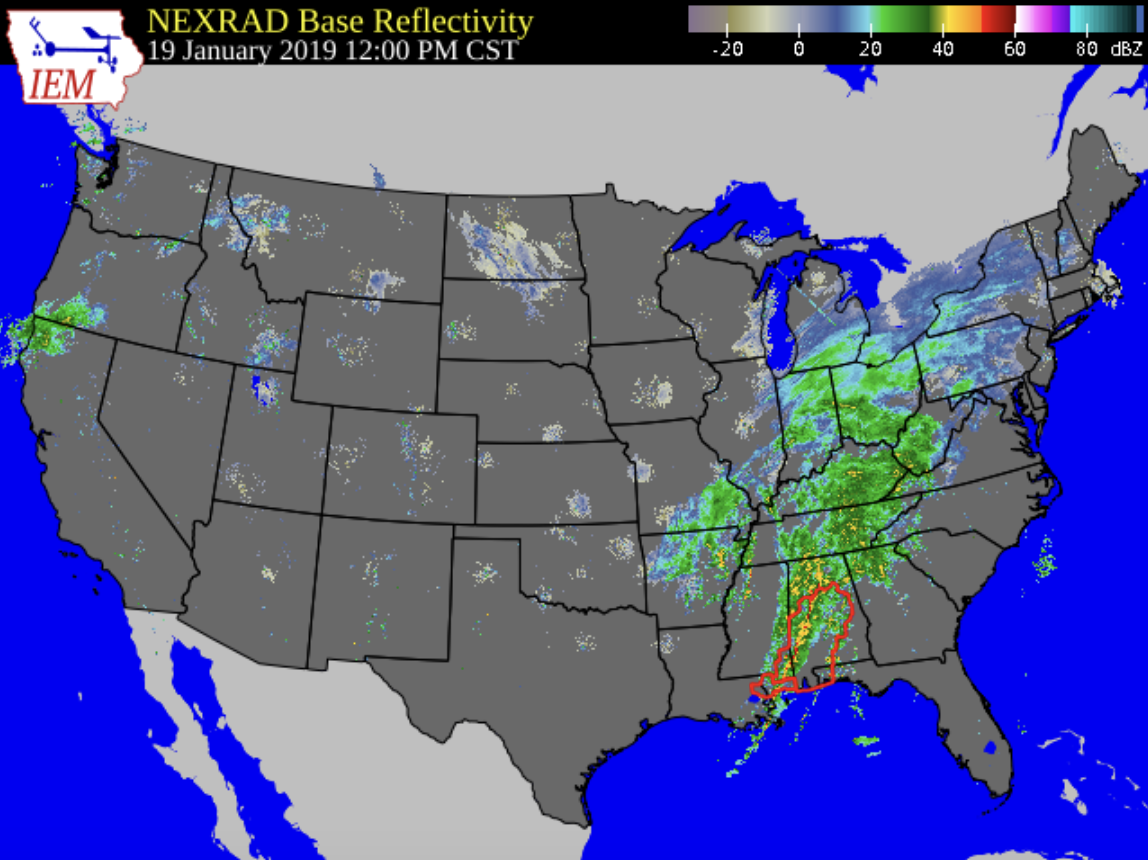
\includegraphics[width=0.49\linewidth]{media/nexrad_2019_01_19_12pm.png}
    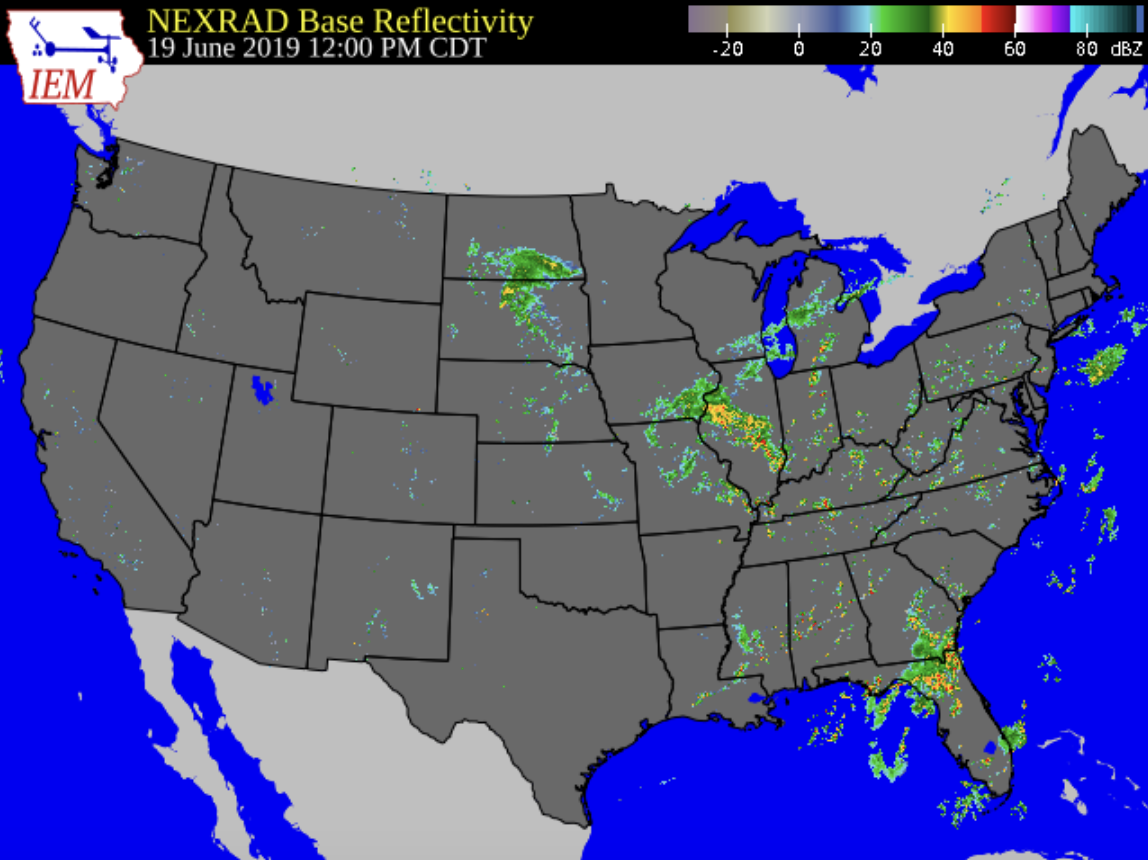
\includegraphics[width=0.49\linewidth]{media/nexrad_2019_06_19_12pm.png}
    \caption{Radar reflectivity maps showing different severities of convective weather from two example days in 2019. The left side shows a more cohesive and globalized convective weather disruption, while the right side shows more sparse and localized disruptions.}
    \label{fig:nexrad-example}
\end{figure}

However, depending on the severity, it may still be possible to consider it localized to a particular sub-network, and consider its aggregated interactions with the rest of the network. Of course, it's often not so simple to just reduce the severity of an event to a single quantity, so we will discuss more about what exactly severity should mean later along with ways to express it in an interpretable manner. Another related factor that can be considered is the frequency of the event, as the processes for handling an area with poor visibility conditions all year round should be very different from planning for much rarer large-scale catastrophic storms.

One point to note is that a localized weather impact can still have network level effects, because of the responses that might be put into place. For example, if a particular node in the network, i.e. a single airport, is under poor weather conditions that make it difficult to service the originally scheduled flow of incoming flights, traffic management initiatives (TMIs) may be implemented to regulate air traffic at a network level. As shown in \cref{fig:gdp-example} from \cite{faa_status_2025}, this is known as a Ground Delay Program (GDP), and shows how issues at a single node of the overall traffic network can easily be broadcast to its neighbors and the rest of the network.

\begin{figure}[htb!]
    \centering
    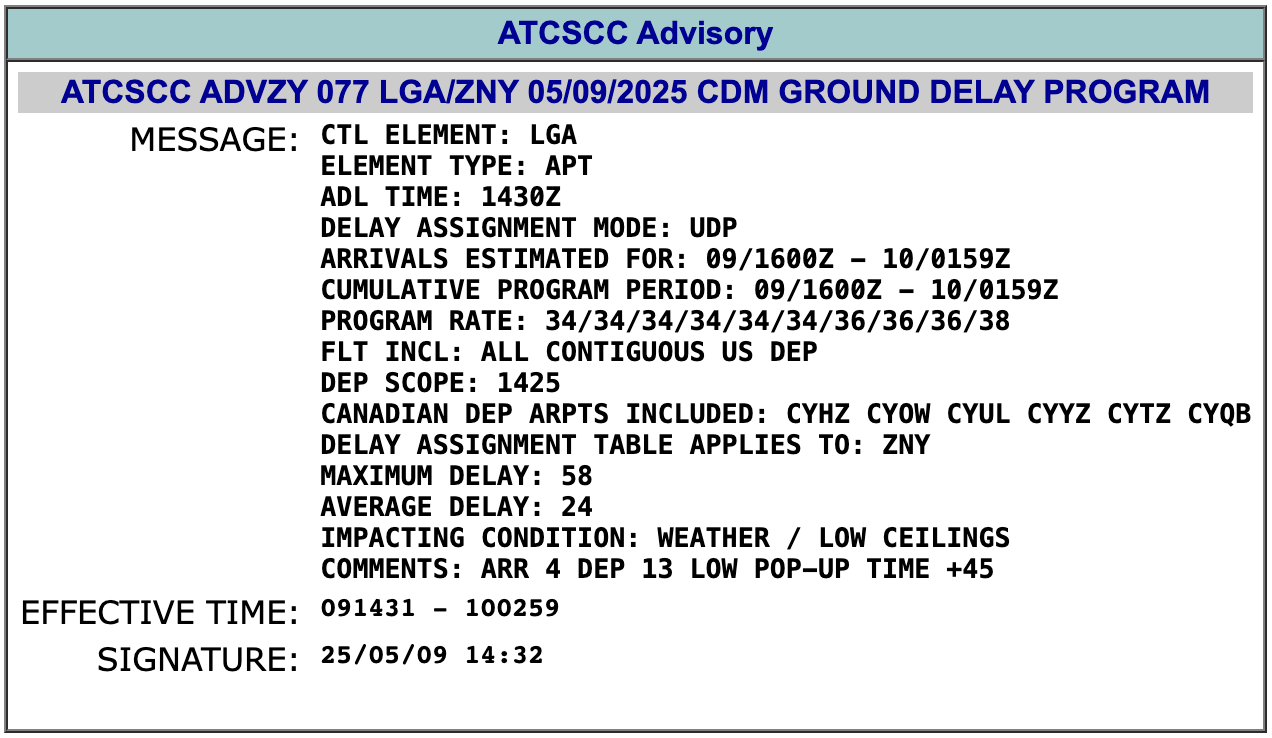
\includegraphics[height=2.2in]{media/gdp_advisory.png}
    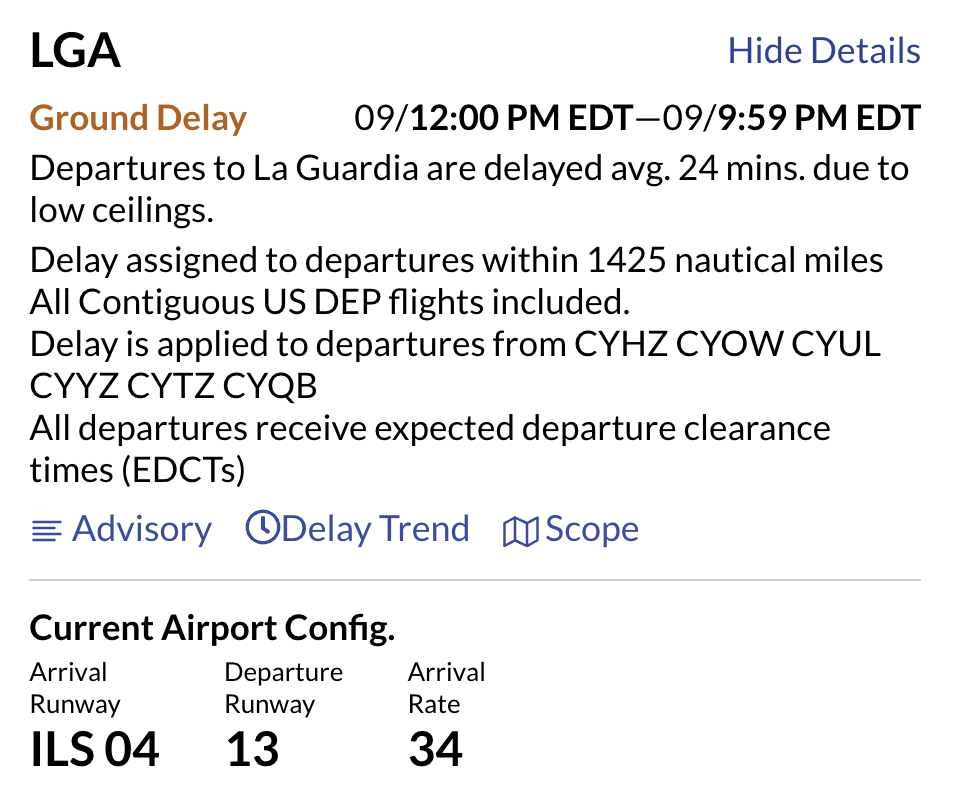
\includegraphics[height=2.2in]{media/gdp_meaning.png}
    \caption{GDP applied to flights headed to LGA due to weather on May 9th, 2025.}
    \label{fig:gdp-example}
\end{figure}

For completeness, we will also describe some other common TMIs, roughly sorted by their general purpose. First, initiatives to create space, both physically and temporally, between aircraft generally fall into one of several categories. Altitude-based TMIs may be used to separate traffic flows close to each other, by imposing altitude restrictions at various phases of a flight, both at arrival and departure, as well as en-route. Miles-in-trail and Minutes-in-trail (MINIT) work along a slightly different axis, where aircraft along a common flow of traffic are directed to be spaced out by at least some minimum physical or temporal separation, depending on what sensor information is available and the spacing required \cite{faa_tfm_prez_2009}.

Other traffic initiatives work more directly to manipulate the timing of arrival and departure phases of flights. For example, fix balancing may change these times to even out traffic at the arrival or departure endpoint of a flight. Similarly, flights may be held on the ground at the departure endpoint, as we saw earlier with GDPs, and also in the air at the arrival endpoint, which is known as airborne holding. The locations of flight endpoints might also changed by reroutes or diversions, which may happen both before departure and en-route. In some more extreme cases, Ground Stops (GSs), where certain flights are held on the ground until the GS is lifted instead of just delayed as in GDPs, may be even necessary \cite{faa_tmi_2024}.

Although we will not discuss these TMIs in more detail, the main takeaway is that even localized disruptions can become globalized because of the actions taken as a result of necessary responses. Therefore, it is natural to first separate our disruptions into two categories. We will say that disruptions that originate completely outside of the system and are, such as weather effects reducing an airport's capacity, are exogenous disruptions. On the other hand, disruptions that are created as a result of actions taken within the system, such as flight delays due to the implementation of GDP in response to an exogenous effect, will be referred to as endogenous disruptions. While these two can be related, as in our GDP example, the effects of disruptions only accumulate in one direction: exogenous disruptions can cause and exacerbate endogenous disruptions, but not the other way around. Because of this, it makes sense to break up observed disruptions into causally linked components and work out their dependency structure, as we will see later.

\subsection{Other Factors}

As we saw earlier, exogenous disruptions from natural events like convective weather can lead to endogenous disruptions from traffic management initiatives raised in response. One natural question to ask is then, how other stakeholders may be affected by both of these. We can also classify these as endogenous effects, but it makes sense to distinguish who is responsible for said effect, which may be traffic managers, or airlines. In the case of airlines, there is potential for further disruptions that are a result of less than optimal processes in place to respond to their flights being delayed. For example, this could be not having allocated crew and fleet resources in a sufficiently robust manner \cite{dot_penalizes_2023}, or being unable to adapt quickly enough to changing situations. In this sense, we can see that there is also a sort of response to the disruptions here, only this time on the part of airlines instead of traffic managers. 

For instance, one common response is to cancel flights that the airline believes they will be unable to service, for some reason or another \cite{bts_causes_2024}. Although airlines do sort of exert pressure on traffic managers through the demand they create with scheduled flight operations, during a disruptive event on a day to day basis, their actions are still more in response to what happens from ATM actions. Therefore, with this dependency structure in mind, we can see that we have several steps that occur mostly in order conceptually, which are weather, traffic manager responses, then airline responses. 

At each step, we can accumulate more severity, so to speak. The weather events initiate disruptions, traffic managers may or may not respond optimally, and then airlines may or may not respond optimally to what the situation is once it ends up at them. This order is important because failures often only occur above some threshold level of severity, in some sense, so there may be less than optimal processes further along the pipeline that are not discovered because the processes before them are doing alright, but in slightly more severe events may manifest and lead to serious unexpected issues. 

We will also note that there are other factors that could fall under the exogenous step, and be treated as a given that is not really a response to anything necessarily in the network. For example, airports undergoing large construction projects may have reduced performance compared to normal operation \cite{faa_construction_2025}. Staffing issues for facilities within the NAS may also pose challenges that may not be immediately fixable \cite{faa_newark_staffing_2025}. Similarly to weather, it may be difficult to exactly represent how these other factors may affect different parts of the network. 

\subsection{Taxonomy Outline}

Now that we have a better idea of the flow of disruptions and associated responses in our system, we can begin to put together a taxonomy of disruptions and responses, which will help us better understand how historical failures, which may seem very different at first glance, are intrinsically related below the surface. It is important to stress that this will not attempt to be any sort of comprehensive classification, but rather a collection of ideas from our reasoning above placed in a coherent framework to motivate further study.

\paragraph{Dependency structures} First, we need to generate a dependency structure for the major events that combine to form the overall observed disruption. This should incorporate both exogenous and endogenous effects. For the exogenous disruptions, since we consider them to be essentially uncontrollable environment parameters, we should also consider the frequency and severity of the event, both expected based on domain knowledge, and historical based on past data, if any. 

\paragraph{Severity} We can further break down severity into a few different parts. The first is the persistence of the event, or how long it was in effect. Longer events are generally of more concern than shorter ones, given the same pure severity level. Here, by pure severity, we are just referring to the direct instantaneous effect of the event without considering any temporal aspects. In practice, however, pure severity and length tend to be relatively well correlated. Moving on from temporal considerations, a third aspect to consider is the spatial size of the event. Roughly speaking, this would refer to whether the event was local to a single node and a just few nearby nodes, or if spanned a significant part of the overall network. If the event can be split into several sparse, more localized components, then it may be more natural to consider it that way instead. There are other things that could be considered here, but for now, these are most relevant.

\paragraph{Frequency} In terms of frequency, we are both interested in frequency in the usual sense, or how often said event occurs, and what we will call predictability. This is essentially just to say that there is a difference between infrequent events that happen completely randomly, and infrequent events that occur on a regular basis. Likewise, not all frequent events are created equal. For example, we might know that certain months are more prone to severe storms than others, and this can be something that is modeled in. 

\paragraph{Simplified example} Let us use a slight extension of our guiding example in \cref{ch:atrds} to give us something concrete to work with. In this hypothetical scenario, we will suppose that due to an ongoing weather event at LGA, the airport arrival and departure capacities were greatly lowered, and a ground delay was implemented for scheduled incoming flights. For one airline, these delays propagated throughout the network, because of insufficient fleet reserves, and led to a large number of canceled flights for the day. The weather event was unusually severe and persistent, and was not something that had been commonly seen up until now. However, it was mostly localized to the airspace around LGA, and did not directly affect the operations of most of the other airports in the network that were not nearby.

In this simplified example, we can separate the overall disruption into three components that follow a linear dependency structure. First, the weather event reducing capacity at LGA is the exogenous disruption. Then, the ground delay is an endogenous disruption generated in response. Finally, the airline flight cancellations is the third component. In our weather event itself, we can see that it is relatively well localized, but is severe both in terms of pure severity and persistence. The weather event is infrequent, and since it is a newly observed type of event, we consider it to be unpredictable by default. 

Moving on from categorizing the initial exogenous disruption, we can also analyze the accumulated disruption as we move through the dependencies that ultimately led to the hypothetical failure. Here, there are a few groups of possibilities. One would be that the traffic management was done optimally, in which case this failure would reveal a weakness in the airline processes that had not been exposed up until this point, due to a continuance of only nominal conditions. Similarly, it is also possible that the airline responded optimally within their constraints, and that improvements could have been made to the traffic management response, and of course, everything in between, as real scenarios are generally not so cut and dry. 

\paragraph{Stakeholder perspectives} Assessing this allocation of accumulated disruption across nodes in the dependency graph can be challenging and often subjective, though not necessarily impossible. However, we will instead focus on a variational approach, where we assume the perspective of the relevant stakeholder to a particular node, and model the rest of the nodes as autonomous processes acting according to a defined set of behaviors based on prior belief. In our hypothetical example, this could be building a simulation where the airline response can be controlled, but all else are held constant, in order to assess how different strategies might have performed, and if there was any improvement to be made leading up to the failure. We can also consider the entire system to be autonomous, in which case we would arrive at the problem of inferring the initial exogenous disruptions, which is the scenario our work in \cref{ch:atrds} would fall under.

\section{Historical Case Studies}

We will now apply our taxonomy to real historical examples, which may help in motivating the structures and perspectives to build our simulations in mind with. The point is to show that by analyzing these scenarios in this manner, we can also get a better idea of where improvements could be made, so that we can decide which parts of the model should be controllable and which should not, as well as parameters to represent the disruption.


\paragraph{Chronically delayed flights} The Bureau of Transportation Statistics defines chronically delayed flights as ``flights with more than 50\% delayed arrivals of more than 30 minutes'' \cite{bts_chronic}. Historically, legal and punitive action, of hundreds of thousands of dollars in penalties, have been taken against carriers such as Southwest Airlines and Frontier Airlines for operating chronically delayed flights, as these are considered evidence of illegally unrealistic scheduling that can negatively affect both passengers and industry standards \cite{southwest_chronic_2025}. By definition, these are high frequency events that are predictable, at least at the point when they become classified as such. Since the impact on an individual basis is limited to a single flight, they are also low severity, but can add up if it is a common occurrence across an airline's routes. Since this is specifically caused by airline scheduling practices, we don't have an exogenous event or traffic management response for risk to accumulate through, therefore our dependency graph only involves the airline. In some sense, the airline's poor scheduling practices could be considered an exogenous event in this case.

\paragraph{Logan snow and ice delays} Next, we return to a more standard exogenous effect from poor weather. At Logan International Airport, snow and ice caused hundreds of flights to be delayed one Saturday in January 2025, even though the storm was relatively localized and not a major event in the surrounding area. A ground delay program was initiated because of the weather to manage capacity. However, because the weather event moved South over time, other nodes began to be affected, which led to thousands more delays and cancellations in later days \cite{nbc_logan_2025}. Here, we can clearly see the dependence structure, progressing linearly from winter weather to traffic management response as a GDP, to disruptions for flights in the network. Note that we can see two aspects of severity here: first, that the storm system had a localized effect mostly contained to a single area, but that same storm system ended up having a much larger effect as it moved and was no longer localized. The storm appeared to be in line with usual winter weather, but is still a relatively infrequent event, so we can say that it is predictable but low frequency.

\paragraph{Newark radar outages} We can also observe a similar effect at a single node, although this time, due to a non-weather effect. In 2025, Newark Liberty International Airport (EWR) suffered multiple incidents of radar and connection outages that caused significant disruption to capacity, as well as staffing issues as a secondary effect. These events sometimes only lasted a short period of time, but still eventually led to widespread effects as the disruption propagated throughout the network \cite{apnews_newark_2025}. This scenario is similar to the previous one. However, one fundamental difference is that weather cannot be addressed directly, as it is something that is totally out of our control, while air traffic control systems in need of repair is something that can be done. Another key difference is that storms are generally higher length events, while we can see here that radar outages may have much shorter length.

\paragraph{Southwest scheduling crisis} Finally, we once again turn our attention to the Southwest Airlines scheduling crisis during winter storms in 2022, which we've discussed earlier multiple times \cite{cnn_southwest_2022}. We note that the exogenous event in this case was low frequency but relatively predictable. The severity was high, both in terms of duration length, pure severity, and spatial size. It's difficult to say if the traffic management response accumulated significant severity, but because Southwest was specifically affected far more than other airlines, it is likely that it was more of an issue with their response specifically. This sort of exogenous event that exposes some weakness in an airline's systems also has shown up often in the past, such as with Southwest again in 2021 \cite{cnn_southwest_2021}, American Airlines in 2018 \cite{usatoday_aa_2018}, and Delta in 2017 \cite{cnn_delta_2017}. A recurring theme seems to be that difficulties in IT systems tend to exacerbate issues, which means that for these cases, it would make sense to focus on airline responses as a controllable aspect of the simulation. Additionally, incorporating reaction speed could be a reflection of how well the IT systems work, and we would also expect to see that a more reactive response would likely perform better than one that is slower. 

\paragraph{Delta IT outages} We will also include one more related example of Delta in 2024, where the disruption was directly in IT systems as a major outage during a failed CrowdStrike software update, leading to thousands of canceled flights \cite{cnbc_delta_crowdstrike_2024}. Although this is related to the previous examples we just discussed, it is slightly different in that the disruption was essentially exogenous, but bypassed every other step to directly affect airline operations. In cases like these where reacting is not particularly feasible, we could instead try to focus on modeling recovery after the fact.

\section{Summary}

In this chapter, we first introduced the primary object we are interested in, the National Airspace System, and covered the hierarchical structure through which air traffic control and management operate within it. Additionally, we briefly went over simulation considerations, and discussed what use cases current state-of-the-art simulators may not necessarily cover completely. Then, we introduced a taxonomy of weather disruptions and responses, breaking them down into dependency structures and multi-faceted notions of frequency of severity, as well as stakeholder perspective. Finally, we applied our taxonomy to a few real world historical scenarios for demonstration.